\chapter{Solución propuesta}

En el presente capítulo se presenta la propuesta de diseño de la solución para el problema de investigación abordado en el presente trabajo, así como su implementación.

\section{Diseño de la solución propuesta} \label{Diseño de la solución propuesta}
En diseño de la solución propuesta se plantean las herramientas utilizadas y los pasos seguidos para la solución propuestas.

Las herramientas utilizadas en la presente investigación se muestran en el cuadro \ref{tab:Herramientas utilizadas}.

\begin{table}[H]
	{\centering
		\caption{Herramientas utilizadas.}
		\begin{tabular}{|c|c|c|}
			\hline 
			Herramienta & Versión & URL\\
			\hline
			\texttt{Python} & 3.8.8 & \url{https://www.python.org/}\\
			\hline
			\texttt{Jupyter Notebook} & 6.3.0 & \url{https://jupyter.org/}\\
			\hline
			\texttt{Imageio} & 2.9.0 & \url{https://imageio.readthedocs.io/}\\
			\hline
			\texttt{Latextable} & 0.2.1 & \url{https://pypi.org/project/latextable/}\\
			\hline
			\texttt{Matplotlib} & 3.3.4 & \url{https://matplotlib.org/}\\
			\hline
			\texttt{NumPy} & 1.20.1 & \url{http://www.numpy.org/}\\
			\hline
			\texttt{Pandas} & 1.2.4 & \url{https://pandas.pydata.org/}\\
			\hline
			\texttt{Seaborn} & 0.11.1 & \url{https://seaborn.pydata.org/}\\
			\hline
			\texttt{Scikit-learn} & 0.24.1 & \url{https://scikit-learn.org/}\\
			\hline
			\texttt{SciPy} & 1.6.2 & \url{https://docs.scipy.org/}\\
			\hline
			\texttt{Statsmodels} & 0.12.2 & \url{https://www.statsmodels.org/}\\
			\hline
			\texttt{Texttable} & 1.6.4 & \url{https://pypi.org/project/texttable/}\\
			\hline
		\end{tabular}
		
	\label{tab:Herramientas utilizadas}
	}
\end{table}

\subsection{Recolección de datos}
La primera fase es la recolección de datos. El objetivo es tener un archivo que contenga datos de los niveles de uno o más contaminantes del aire en años recientes y también del mismo lugar tener datos del número de egresos hospitalarios durante esos años.

\subsection{Selección y agrupación de datos}
Después de la recolección de datos se procede a seleccionar que datos van a ser utilizados para los experimentos. Para ello se utiliza \texttt{Python} con la librería \texttt{Pandas} \ref{tab:Herramientas utilizadas} que permite la manipulación de datos. 
Para la selección y agrupación de datos se sigue el procedimiento mostrado en la figura \ref{alg:a1}.

\begin{algorithm}
\caption{Selección y agrupamiento de datos}\label{alg:a1}
\begin{algorithmic}[1]
\State $a \leftarrow $ años de los que se obtuvieron datos
\For {$i \in a$}
    \State $contaminantes \leftarrow $ nombre del archivo .csv que contiene los datos de los contaminantes en el año $i$
    \State Leer en $contaminantes$ las columnas fecha y contaminante 
    \State $egresos \leftarrow $ nombre del archivo .csv que contiene los datos de los contaminantes en el año $i$
    \State Leer en $contaminantes$ las columnas fecha, padecimiento y estado
    \State $estado \leftarrow $ estado del que se quieren obtener datos
    \State Seleccionar en $contaminantes$ los datos del $estado$
\EndFor
\end{algorithmic} 
\end{algorithm}

\subsection{Visualización de la evolución de las variables}
Al ya tener seleccionados los datos a utilizar se procede a elaborar gráficos en \texttt{Python} \ref{tab:Herramientas utilizadas} que muestran la evolución de las variables en el tiempo. Para ello se generan los tipos de gráficos discutidos a continuación.

\subsubsection{Series de tiempo}
Se realizan series de tiempo en \texttt{Python} con ayuda de la librería  \texttt{Matplotlib}, \texttt{Scikit-learn} y \texttt{Seaborn} \ref{tab:Herramientas utilizadas}, ya que son herramientas accesibles que ayudan a la generación de este tipo de gráficos. %; en la figura \ref{serie_de_tiempo} se muestra un ejemplo de las series de tiempo generadas.

%\begin{figure}[h!]
%\setcounter{figure}{0} % por culpa de sciposter
%\captionsetup{type=figure} % por culpa de sciposter
%\begin{center}
%   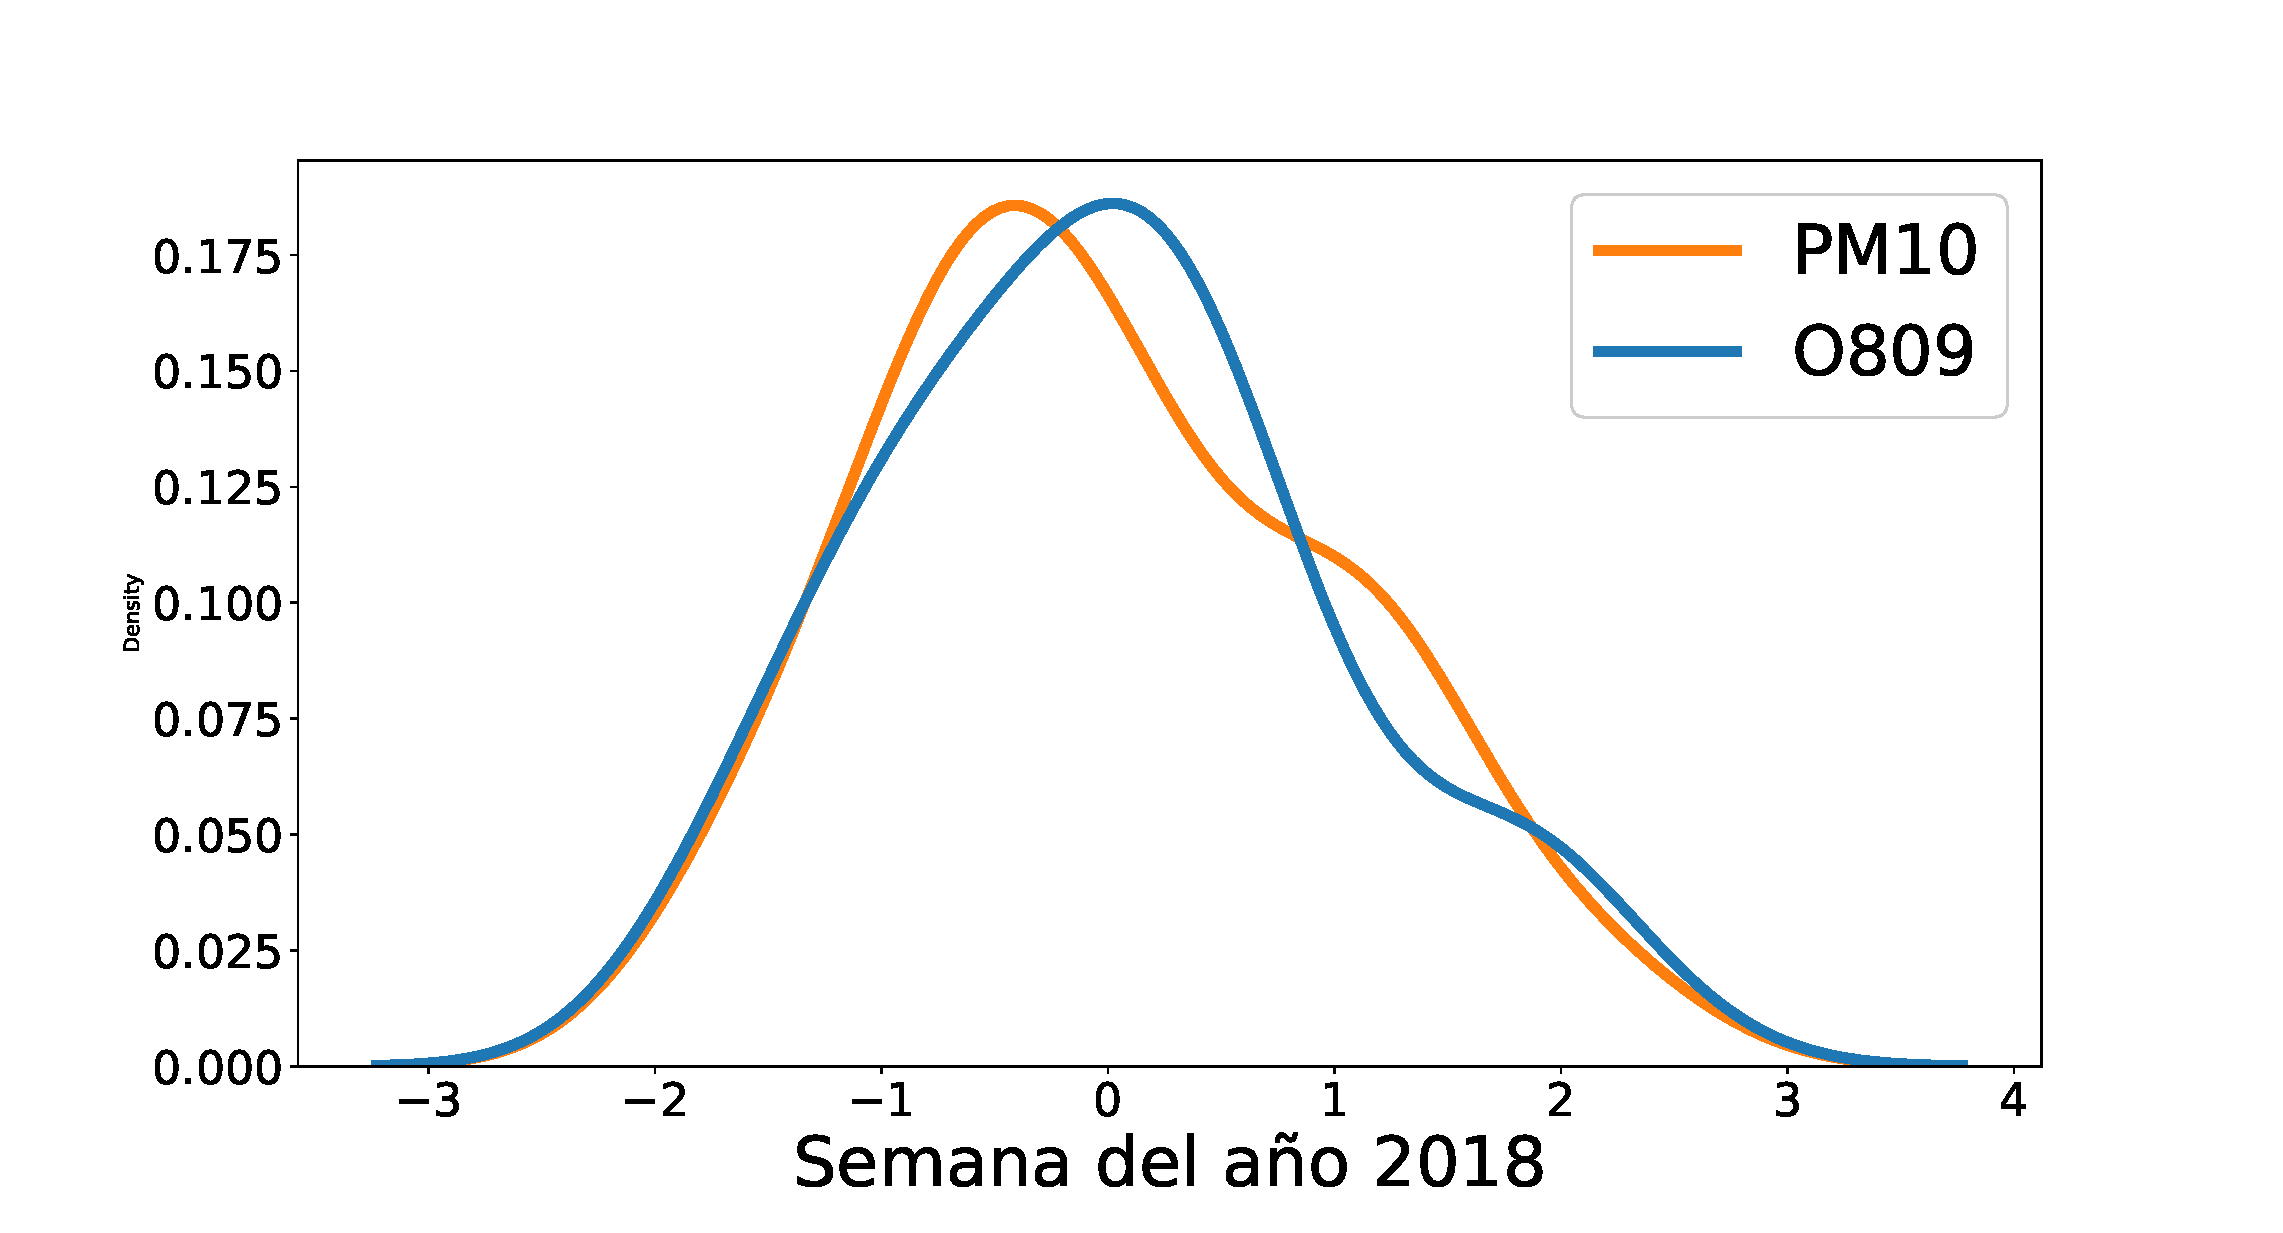
\includegraphics[width=1\textwidth]{PM10_O809_2018.eps}
%   \end{center}
%    \caption[Ejemplo de series de tiempo]{Evolución de los niveles de PM10 y el número de egresos diagnosticados con la CIE O809 en el 2018.}
%    \label{serie_de_tiempo}
%\end{figure}

\subsubsection{Gráficos de radar}
Los gráficos de radar o diagramas de telaraña son otra manera de visualizar un conjunto de datos. Sirven para comparar variables visualizando si existen valores o patrones de evolución en el tiempo similares entre ellas. Es por ello que en el presente trabajo se elaboran gráficos de radar con ayuda de \texttt{Python} y las librerías \texttt{NumPy} y \texttt{Matplotlib} \ref{tab:Herramientas utilizadas}. En la figura \ref{grafico_de_telaraña} se muestra un ejemplo de los gráficos de telaraña generados.

\begin{figure}[h!]
\setcounter{figure}{0} % por culpa de sciposter
\captionsetup{type=figure} % por culpa de sciposter
\begin{center}
   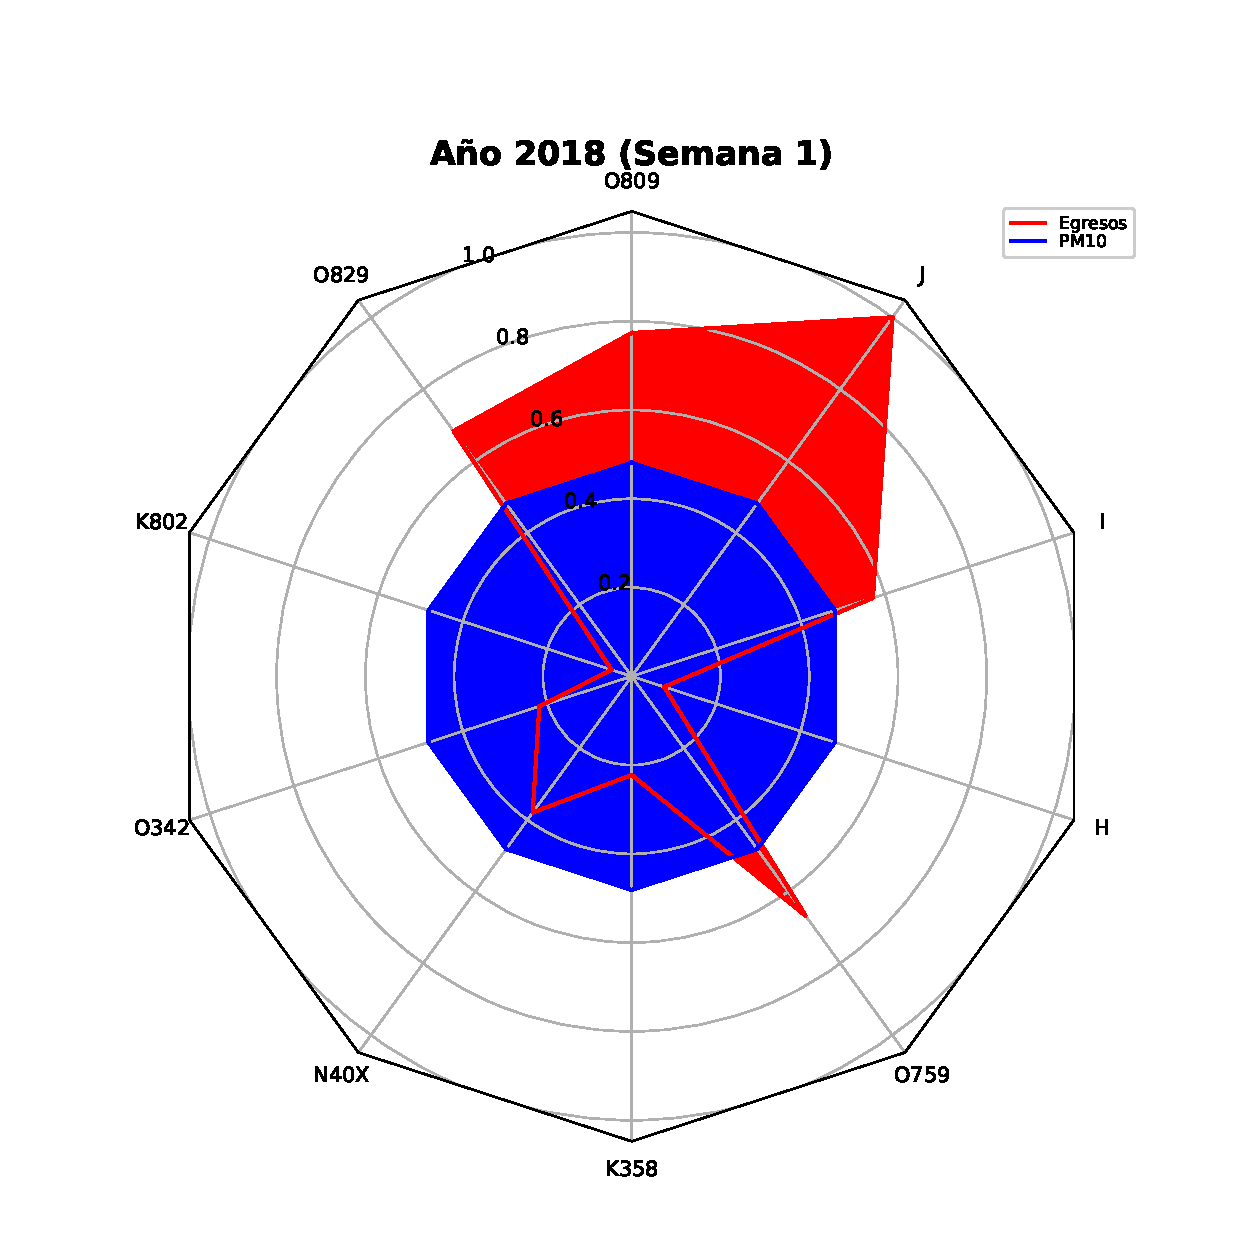
\includegraphics[trim=0 0 0 74,clip,width=1\textwidth]{spiderweb_PM10_2018_1.eps}
   \end{center}
    \caption[Ejemplo de gráfico de radar]{Nivel del contaminante PM10 y egresos por CIE en la semana 1 del año 2018.}
    \label{grafico_de_telaraña}
\end{figure}

\clearpage
\subsection{Implementación de modelos}
Después de haber generado gráficos para la visualización de la evolución de las variables, se procede a generar modelos para el estudio de la relación entre las variables. Para ello se utiliza \texttt{Python} y la librería \texttt{Statsmodels} \ref{tab:Herramientas utilizadas}. Los tipos de modelos generados se discuten a continuación.

\subsubsection{Regresión lineal}
Primeramente se calcula el coeficiente de correlación de Pearson, si el valor de la correlación se encuentre entre -1 y 1 significa que existe una dependencia lineal y que existe sustento para el modelo de regresión lineal. El modelo de regresión lineal arroja un valor de $R^2$ que indica en que grado la variable independiente explica la varianza de la variable dependiente. Además, se obtiene el valor $p$ que indica la relevancia del resultado y se obtiene la raíz de error cuadrático medio (RMSE) que indica cuantas unidades se alejan los valores predichos por el modelo de los valores reales, eso ayuda a determinar el error del modelo.

\subsubsection{Regresión lineal múltiple}
En los modelos de regresión lineal múltiple se tiene más de una variable independiente. Al obtener el valor de la correlación entre -1 y 1 para verificar que existe sustento para el modelo de regresión lineal, se procede a generar el modelo de regresión lineal múltiple. El modelo de regresión lineal múltiple arroja un valor de $R^2$ que indica en que grado las variables independientes explican la varianza de la variable dependiente. Además, se obtiene el valor $p$ que indica la relevancia del resultado y se obtiene la raíz de error cuadrático medio (RMSE) que indica cuantas unidades se alejan los valores predichos por el modelo de los valores reales, eso ayuda a determinar el error del modelo.

\section{Implementación de la solución propuesta}
En implementación de la solución propuesta se muestra el desarrollo realizado de los puntos planteados en la sección \ref{Diseño de la solución propuesta}. La figura \ref{Diagrama de flujo de las fases} muestra las fases seguidas para el desarrollo de la solución propuesta, la cual consiste en la generación de visualizaciones y modelos. El desarrollo del presente proyecto se encuentra en el siguiente repositorio Github: \url{https://github.com/selenebpradop/relaciones-contaminantes-salud/}.

\begin{description}
\item{En el fragmento de código \ref{lst:c1} se muestra el proceso realizado para el procesamiento y agrupamiento de los datos en semanas epidemiológicas, esto para que los datos puedan ser utilizados para generar figuras y modelos de regresión lineal.}
\item{El fragmento de código \ref{lst:c2} muestra como es que se generan las series de tiempo, esto después de haber procesado y agrupado los datos.}
\item{El fragmento de código mostrado en \ref{lst:c3} genera una animación de gráficos de radar al ingresarle como parámetros los datos ya procesados y agrupados. Dicha animación es generada en formato .mp4 o .gif para poder visualizar la evolución de las variables por semana del año y contaminante.}
\item{En el fragmento de código \ref{lst:c4} se muestra como son generados los modelos de regresión lineal después de obtener un coeficiente de correlación de Pearson entre -1 y 1.}
\item{El fragmento de código \ref{lst:c5} muestra como se generan los modelos de regresión lineal múltiple después de generar los modelos de regresión lineal individuales. Todos los modelos generados por librería \texttt{Statsmodels} \ref{tab:Herramientas utilizadas} se guardan en formato .tex.}
\end{description}

\begin{figure}[H]
  \resizebox{.75\columnwidth}{!}{
  \begin{tikzpicture}[node distance=2cm, auto]
 \node [cloud] (init) {Inicio};
 \node [block, below of=init] (agrupamiento) {Agrupamiento de datos en semanas epidemiológicas};
 \node [block, below of=agrupamiento] (series) {Generación de las series de tiempo};
 \node [block, below of=series] (spiderweb) {Generación del gráfico de radar};
 \node [block, below of=spiderweb] (correlacion) {Cálculo de la dependencia lineal $\rho$};
 \node [decision, below of=correlacion] (decision1) {$\rho \in [-1,1]$};
 \node [block, left of=decision1, node distance=6cm] (cancell) {Registrar el valor de la correlación};
 \node [block, below of=decision1, node distance=4cm] (rl) {Generación del modelo de regresión lineal};  
 \node [block, below of=rl] (rlm) {Generación del modelo de regresión lineal múltiple};
 \node [cloud, below of=rlm, node distance=2cm] (end) {Fin};
 \path [line] (init) -- (agrupamiento);
 \path [line] (agrupamiento) -- (series);
 \path [line] (series) -- (spiderweb);
 \path [line] (spiderweb) -- (correlacion);
 \path [line] (correlacion) -- (decision1);
 \path [line] (decision1) -- node {no} (cancell);
 \path [line] (cancell) |- (end);
 \path [line] (decision1) -- node {sí} (rl);
 \path [line] (rl) -- (rlm);
 \path [line] (rlm) -- (end);
\end{tikzpicture}}
\caption{Fases del desarrollo de la solución}
\label{Diagrama de flujo de las fases}
\end{figure}

\clearpage
\begin{lstlisting}[language=Python, caption=Procesamiento y agrupamiento de datos, label=lst:c1]
import pandas as pd
from epiweeks import Week, date
from sklearn import preprocessing
import seaborn as sns
import matplotlib.pyplot as plt
import string

columns = ['timestamp', contaminante]
dataframec = pd.read_csv('filled.csv', usecols=columns).dropna()
strfdt = '%d-%b-%y %H'
dataframec['timestamp'] = pd.to_datetime(dataframec['timestamp'], errors = 'coerce', format=strfdt)
dataframec = dataframec.dropna()
dataframec = dataframec.reset_index(drop=True)
dataframec['timestamp'] = dataframec['timestamp'].apply(lambda x: x.strftime('%Y-%m-%d %H'))
dataframeca = dataframec.loc[dataframec['timestamp'].str.startswith(año)]
dataframeca = dataframeca.reset_index(drop=True)
strfdt = '%Y-%m-%d %H'
dataframeca['timestamp'] = pd.to_datetime(dataframeca['timestamp'], errors = 'coerce', format=strfdt)
dataframeca['sem'] = dataframeca['timestamp'].apply(lambda x: date(x.year, x.month, x.day))
dataframeca['sem'] = dataframeca['sem'].apply(lambda x: Week.fromdate(x))
dataframeca['sem'] = dataframeca['sem'].apply(lambda x: x.week)
colums = ['EGRESO', 'DIAG_INI']
csvegresos = 'EGRESO_' + año + '.csv'
dataframeea = pd.read_csv(csvegresos, usecols=colums).dropna()
dataframeea['EGRESO'] = pd.to_datetime(dataframeea['EGRESO'], errors = 'coerce', format=strfdto)
dataframeea = dataframeea.loc[dataframeea['ENTIDAD'] == entidad]
dataframeea = dataframeea.dropna()
dataframeea = dataframeea.reset_index(drop=True)
numaño = int(año) 
dataframeea['sem'] = dataframeea['EGRESO'].apply(lambda x: date(x.year, x.month, x.day))
dataframeea['sem'] = dataframeea['sem'].apply(lambda x: Week.fromdate(x))
dataframeea['sem'] = dataframeea['sem'].apply(lambda x: x.week)
dataframeea['EGRESO'] = dataframeea['EGRESO'].apply(lambda x: x if(x.year==numaño) else pd.NaT)   
dataframeea = dataframeea.dropna()
dataframeea = dataframeea.reset_index(drop=True)
dataframesca = pd.DataFrame()
dataframesca['sem'] = semanas.index
dataframesca[contaminante] = ''
n = len(semanas.index)
for i in range (n):
    registrossem = dataframeca.loc[dataframeca['sem'] == i+1]
    promediocas = registrossem[contaminante].mean()
    dataframesca[contaminante][i] = promediocas
\end{lstlisting}

\clearpage
\begin{lstlisting}[language=Python, caption=Generación de series de tiempo, label=lst:c2]
import pandas as pd
from epiweeks import Week, date
from sklearn import preprocessing
import seaborn as sns
import matplotlib.pyplot as plt
import string

diagnosticosaño = dataframeea['DIAG_INI'].value_counts()
diagnosticosaño = diagnosticosaño.sort_values(ascending = False)
ciesaño = dataframeea.groupby(['DIAG_INI', 'sem']).count()

s_scaler = preprocessing.StandardScaler()
ind = []
n = len(semanas.index)
for i in range (n):
    ind.append(i+1)
letras = []
for letra in string.ascii_uppercase:
    letras.append(str(letra))
# Se inicia un contador para controlar la cantidad de graficos a generar
cont = 0
maximo = 10
mindividuales = 7

# Proceso de generación de las figuras
print('\n' + año)
for name in diagnosticosaño.index:
    if cont < maximo:
        dataframegraficoacc = pd.DataFrame()
        dataframegraficoacc[contaminante] = dataframesca[contaminante]
        dataframegraficoacc = dataframegacc.reindex(ind)
        if cont < mindividuales:
            dataframegacc[name] = ciesaño['EGRESO'][name]
            for i in range (n):
                dataframegacc[contaminante][i+1] = dataframesca[contaminante][i]
            col_names = [contaminante, name]    
        else:
            nameg =  letras[cont]
            ciesagrupadas = dataframeea.loc[dataframeea['DIAG_INI'].str.startswith(nameg)]
            ciesagrupadas = ciesagrupadas['sem'].value_counts()
            dataframegacc[nameg] = ciesagrupadas
            for i in range (n):
                dataframegacc[contaminante][i+1] = dataframesca[contaminante][i]
            col_names = [contaminante, nameg]
        df_s = s_scaler.fit_transform(dataframegacc)
        df_s = pd.DataFrame(df_s, columns=col_names)
        fig, ax = plt.subplots(ncols=1, figsize=(20, 8))
        print('\n' + col_names[0] + ' & ' + col_names[1])
        ax.set_title('Contaminante ' + col_names[0] + ' & CIE ' + col_names[1])
        ax.set_xlabel('Semana del año ' + año)
        sns.kdeplot(data=df_s)
        plt.savefig(contaminante + '/' + col_names[0] + '&' + col_names[1] + '_' + año + '.jpg', format='jpg')
        plt.show()
    cont = cont+1
\end{lstlisting}

\clearpage
\begin{lstlisting}[language=Python, caption=Generación de graficos de radar, label=lst:c3]
def create_spiderwebs(datasets, labels, lenlines, title, titles, spoke_labels, colors, typeframe, outputtype):

    N1 = len(datasets)
    N2 = len(labels)
    N = int(N1/N2)
    theta = radar_factory(N, frame=typeframe)
    i=0
    filenames = []
    for titlespiderweb in titles:
        fig, axs = plt.subplots(figsize=(8, 8), subplot_kw=dict(projection='radar'))
        fig.subplots_adjust(wspace=0.5, hspace=0.20, top=0.85, bottom=0.05)
        ax = axs
        ax.set_title(titlespiderweb, weight='bold', size='medium', position=(0.5, 0.5), horizontalalignment='center', verticalalignment='center', fontsize=16)
        for y in range(N2):
            dataspider = []
            xx = y
            for yy in range(N):
                currentdata = datasets[xx]
                number = currentdata[i]
                nmin = min(currentdata);
                nmax = max(currentdata);
                r = nmax - nmin
                x = (number-nmin)/r
                yyy = lenlines*x
                dataspider.append(yyy)
                xx = xx + N2
            ax.plot(theta, dataspider, color=colors[y])
            ax.fill(theta, dataspider, facecolor=colors[y], alpha=0.05)
        ax.set_varlabels(spoke_labels)
        ax = axs
        legend = ax.legend(labels, loc=(0.9, .95), labelspacing=0.1, fontsize='small')
        i=i+1
        filename = 'spiderweb' + '_' + title + '_' + str(i) + '.jpg'
        filenames.append(filename)
        plt.savefig(filename, format='jpg')
    
    # Generate a GIF
    if(outputtype == 'gif'):
        with imageio.get_writer(title + '.gif', mode='I', duration=1) as writer:
            for filename in filenames:
                image = imageio.imread(filename)
                writer.append_data(image)
    # Generate a .mp4 video
    if(outputtype == 'video'):
        img_array = []
        for filename in filenames:
            img = cv2.imread(filename)
            height, width, layers = img.shape
            size = (width,height)
            img_array.append(img)        
        out = cv2.VideoWriter(title + '.mp4',cv2.VideoWriter_fourcc(*'MP4V'), 1, size)
        for i in range(len(img_array)):
            out.write(img_array[i])
        out.release()
\end{lstlisting}

\clearpage
\begin{lstlisting}[language=Python, caption=Generación de los modelos de regresión lineal, label=lst:c4]
# Gráfico
fig, ax = plt.subplots(figsize=(6, 3.84))
datos.plot(
    x    = col_names[0],
    y    = col_names[1],
    c    = 'firebrick',
    kind = "scatter",
    ax   = ax
)
ax.set_title('Contaminante ' + col_names[0] + ' & CIE ' + col_names[1])
# Correlación lineal entre las dos variables
corr_test = pearsonr(x = datos[col_names[0]], y =  datos[col_names[1]])
# División de los datos en train y test
X = datos[[col_names[0]]]
y = datos[col_names[1]]
X_train, X_test, y_train, y_test = train_test_split(
    X.values.reshape(-1,1),
    y.values.reshape(-1,1),
    train_size   = 0.8,
    random_state = 1234,
    shuffle      = True
)
X_train = sm.add_constant(X_train, prepend=True)
modelo = sm.OLS(endog=y_train, exog=X_train)
modelo = modelo.fit()
if(modelo.pvalues[1]>0.05):
    exclude_p.append(col_names[1])
# Intervalos de confianza para los coeficientes del modelo
modelo.conf_int(alpha=0.05)
# Predicciones con intervalo de confianza del 95%
pred = modelo.get_prediction(exog = X_train).summary_frame(alpha=0.05)
pred.head(4)        
# Predicciones con intervalo de confianza del 95%
pred = modelo.get_prediction(exog = X_train).summary_frame(alpha=0.05)
pred['x'] = X_train[:, 1]
pred['y'] = y_train
pred = pred.sort_values('x')
# Gráfico del modelo
fig, ax = plt.subplots(figsize=(6, 3.84))
ax.set_title('Contaminante ' + col_names[0] + ' & CIE ' + col_names[1])
ax.set_xlabel(col_names[0])
ax.set_ylabel(col_names[1])
ax.scatter(pred['x'], pred['y'], marker='o', color = "gray")
ax.plot(pred['x'], pred["mean"], linestyle='-', label="OLS")
ax.plot(pred['x'], pred["mean_ci_lower"], linestyle='--', color='red')
ax.plot(pred['x'], pred["mean_ci_upper"], linestyle='--', color='red')
ax.fill_between(pred['x'], pred["mean_ci_lower"], pred["mean_ci_upper"], 0.1)
ax.legend()
# Error de test del modelo 
X_test = sm.add_constant(X_test, prepend=True)
pred = modelo.predict(exog = X_test)
rmse = mean_squared_error(
    y_true  = y_test,
    y_pred  = pred,
    squared = False
)
\end{lstlisting}

\clearpage
\begin{lstlisting}[language=Python, caption=Generación de los modelos de regresión lineal múltiple, label=lst:c5]
corr_matrix = datarlm.corr(method='pearson')
corr_mat = corr_matrix.stack().reset_index()
corr_mat.columns = ['variable_1','variable_2','r']
corr_mat = corr_mat.loc[corr_mat['variable_1'] != corr_mat['variable_2'], :]
corr_mat['abs_r'] = np.abs(corr_mat['r'])
corr_mat = corr_mat.sort_values('abs_r', ascending=False)
tidy_corr_matrix = (corr_matrix).head(10)
# Heatmap matriz de correlaciones
fig, ax = plt.subplots(nrows=1, ncols=1, figsize=(4, 4))
sns.heatmap(
    corr_matrix,
    annot     = True,
    cbar      = False,
    annot_kws = {"size": 8},
    vmin      = -1,
    vmax      = 1,
    center    = 0,
    cmap      = sns.diverging_palette(20, 220, n=200),
    square    = True,
    ax        = ax)
ax.set_xticklabels(
    ax.get_xticklabels(),
    rotation = 45,
    horizontalalignment = 'right',)
ax.tick_params(labelsize = 10)
# División de los datos en train y test
X = datarlm[spoke_labels]
y = datarlm[contaminante]
X_train, X_test, y_train, y_test = train_test_split(
    X,
    y.values.reshape(-1,1),
    train_size   = 0.8,
    random_state = 1234,
    shuffle      = True)
# Creación del modelo utilizando matrices como en scikitlearn
X_train = sm.add_constant(X_train, prepend=True)
modelo = sm.OLS(endog=y_train, exog=X_train,)
modelo = modelo.fit()
sml = modelo.summary().as_latex()
namefile = 'modelos_latex/' + 'regresion_lineal_multiple_' + contaminante + '_' + año + '.tex'
f = open(namefile, 'w')
with open(namefile, 'w') as f:
    f.write(sml)
# Diagnóstico errores (residuos) de las predicciones de entrenamiento
y_train = y_train.flatten()
prediccion_train = modelo.predict(exog = X_train)
residuos_train   = prediccion_train - y_train
# Predicciones con intervalo de confianza 
predicciones = modelo.get_prediction(exog = X_train).summary_frame(alpha=0.05)
predicciones.head(4)
# Error de test del modelo 
X_test = sm.add_constant(X_test, prepend=True)
rmse = mean_squared_error(
    y_true  = y_test,
    y_pred  = modelo.predict(exog = X_test),
    squared = False)
\end{lstlisting}
